%
% This is the LaTeX template file for lecture notes for ADS Zhejiang University.  
% When preparing LaTeX notes for this class, please use this template.
%
% To familiarize yourself with this template, the body contains
% some examples of its use.  Look them over.  Then you can
% run LaTeX on this file.  After you have LaTeXed this file then
% you can look over the result either by printing it out with
% dvips or using xdvi.
%
% This template is based on the template for Prof. Sinclair's CS 270.

\documentclass[twoside]{article}
\usepackage{CJKutf8}
\usepackage{multirow}
%\usepackage{graphics}
\usepackage{lineno}
\usepackage{caption}
% \linenumbers
\usepackage{subfig}
\usepackage{graphics}
\usepackage{geometry}

\usepackage{forest,amsmath}
\usepackage{enumerate}
\geometry{left=2.5cm,right=2cm,top=2.5cm,bottom=2.5cm}

%\setlength{\oddsidemargin}{0.25 in}
%\setlength{\evensidemargin}{-0.25 in}
%\setlength{\topmargin}{-0.6 in}
%\setlength{\textwidth}{6.5 in}
%\setlength{\textheight}{8.5 in}
%\setlength{\headsep}{0.75 in}
\setlength{\parindent}{0 in}
\setlength{\parskip}{0.1 in}

\usepackage{threeparttable}
\usepackage{listings}
\usepackage{color}
\renewcommand\lstlistingname{Quelltext} % Change language of section name
\lstset{ % General setup for the package
    language= C,
    basicstyle=\small\sffamily,
    basicstyle=\ttfamily,
    numbers=left,
     numberstyle=\tiny,
    frame=tb,
    breaklines,
    tabsize=4,
    columns=fixed,
    showstringspaces=false,
    showtabs=false,
    keepspaces,
    commentstyle=\color{red},
    keywordstyle=\color{blue}
}
\usepackage{fontspec}
\newfontfamily\JB{JetBrains Mono}
% \setmonofont{JetBrains Mono}[Contextuals = Alternate,
%     Ligatures = TeX, ]
\usepackage[colorlinks,
            linkcolor=blue,       %%修改此处为你想要的颜色
            anchorcolor=blue,  %%修改此处为你想要的颜色
            citecolor=blue,        %%修改此处为你想要的颜色,例如修改blue为red
            ]{hyperref}
% \usepackage{clrscode3e}
\usepackage{algorithmicx}
\usepackage{algpseudocode}
\usepackage{algorithm}
\renewcommand{\algorithmicrequire}{\textbf{Input:}}
\renewcommand{\algorithmicensure}{\textbf{Output:}}
\makeatletter
\newenvironment{breakablealgorithm}
  {% \begin{breakablealgorithm}
   \begin{center}
     \refstepcounter{algorithm}% New algorithm
     \hrule height.8pt depth0pt \kern2pt% \@fs@pre for \@fs@ruled
     \renewcommand{\caption}[2][\relax]{% Make a new \caption
       {\raggedright\textbf{\ALG@name~\thealgorithm} ##2\par}%
       \ifx\relax##1\relax % #1 is \relax
         \addcontentsline{loa}{algorithm}{\protect\numberline{\thealgorithm}##2}%
       \else % #1 is not \relax
         \addcontentsline{loa}{algorithm}{\protect\numberline{\thealgorithm}##1}%
       \fi
       \kern2pt\hrule\kern2pt
     }
  }{% \end{breakablealgorithm}
     \kern2pt\hrule\relax% \@fs@post for \@fs@ruled
   \end{center}
  }
\makeatother

% Use these for theorems, lemmas, proofs, etc.
\newtheorem{theorem}{Theorem}[theorem]
\newtheorem{lemma}[theorem]{Lemma}
\newtheorem{proposition}[theorem]{Proposition}
\newtheorem{claim}[theorem]{Claim}
\newtheorem{corollary}[theorem]{Corollary}
\newtheorem{definition}[theorem]{Definition}
\newenvironment{proof}{{\bf Proof:}}{\hfill\rule{2mm}{2mm}}

% **** IF YOU WANT TO DEFINE ADDITIONAL MACROS FOR YOURSELF, PUT THEM HERE:

\begin{document}
\begin{CJK*}{UTF8}{gbsn}
%FILL IN THE RIGHT INFO.
%\lecture{**LECTURE-NUMBER**}{**DATE**}{**LECTURER**}{**SCRIBE**}
%\lecture{1}{Project Name}{Deshi Ye}{Student 1, Student 2, 学生3}
%\footnotetext{These notes are partially based on those of Nigel Mansell.}
\title{Shortest Path Algorithm with Heaps}
\author{Group number: Jiefeng Wu \and Jiajun Qin \and Wenjie Huang}
\maketitle
% **** YOUR NOTES GO HERE:

% Some general latex examples and examples making use of the
% macros follow.  
%**** IN GENERAL, BE BRIEF. LONG SCRIBE NOTES, NO MATTER HOW WELL WRITTEN,
%**** ARE NEVER READ BY ANYBODY.
\begin{abstract}
This report explores the performance of various heap data structures in optimizing Dijkstra's shortest path algorithm.  The importance of the problem is highlighted, as Dijkstra's algorithm is a fundamental algorithm in graph theory with widespread applications in fields such as transportation networks, computer networking, and social networks.  The methods used in the report include a thorough analysis of the time and space complexity of the algorithm using different heap data structures, including binary heaps, leftist heaps, binomial heaps, and Fibonacci heaps.  Fibonacci heaps offer the best theoretical time and space complexity for Dijkstra's algorithm, with a time complexity of O$(E + V \log V)$ and a space complexity of $O(V)$.  However, in practice, the high constant factors associated with the Fibonacci heap operations may impact its performance.  Therefore, it is important to consider other factors such as the size and structure of the graph, other heaps like leftist heap, binomial heap can also be taken consideration into, too. The implications and significance of this project are discussed, including how this information can be applied in real-world scenarios to improve the efficiency and accuracy of graph-based computations.  Overall, this report provides valuable insights for researchers and practitioners who are looking to optimize Dijkstra's algorithm using the most efficient heap data structures.
\end{abstract}

\section{Introduction}

Shortest path problems are classic and common problems in graph theory. One of the most important algorithms for the shortest path problems is Dijkstra, which we can optimize by min-priority queue. Therefore, the goal of the project is to find the best data structure for the Dijkstra's algorithm.  
% Problem description, purpose of this report, and (if any) background of the data structures and the algorithms.  Be concise.

\section{Data Structure / Algorithm Specification}

\subsection{Data Structures For Graph Representation}

As we all know, the comman data structures for graph representation are adjacency list, adjacency matrix and incidence matrix and so on.

Concering the size of nodes(can be at most 23,947,347) and the size of edges(at most 58,333,344), we choose adjacency list\cite{666} as our data structure for graph representation, with the space complexity of $O(|V|+|E|)$, which is good for a sparse graph.  

For convenience, we use the STL \verb|vector| to achieve adjacency list, which is a container in C++. Every node $v$ has a \verb|vector| which stores the adjacency node, indicating there is an edge starting from $v$. If the edge has values, we can set \verb|struct| as the elements of \verb|vector|, with the attributes of nodes and the edge values.

\subsection{The Algorithm For the Shortest Path Problems -- Dijkstra}

Dijkstra's algorithm\cite{002} is an algorithm for finding the shortest paths between nodes in a weighted graph. It is usually used for solving single-source problems.  

\subsubsection{Algorithm Procedure}
\begin{enumerate}
    \item Mark all nodes unvisited. Create a set of all the unvisited nodes called the unvisited set.
    \item Assign to every node a tentative distance value: set it to zero for our initial node and to infinity for all other nodes. During the run of the algorithm, the tentative distance of a node v is the length of the shortest path discovered so far between the node v and the starting node.
    \item For the current node, consider all of its unvisited neighbors and calculate their tentative distances through the current node. Compare the newly calculated tentative distance to the one currently assigned to the neighbor and assign it the smaller one.
    \item When we are done considering all of the unvisited neighbors of the current node, mark the current node as visited and remove it from the unvisited set.
    \item If the destination node has been marked visited or if the smallest tentative distance among the nodes in the unvisited set is infinity, then stop. The algorithm has finished.
    \item Otherwise, select the unvisited node that is marked with the smallest tentative distance, set it as the new current node, and go back to step 3.
\end{enumerate}
The algorithm can be described by the pseudo-code below.  
\begin{breakablealgorithm}
    \begin{algorithmic}[1] 
        \Function{Dijkstra}{Graph, source}
        \For {each vertex $v$ in $Graph.Vertices$}
                    \State $dist[v]\leftarrow \rm{INFINITY}$
                    \State $prev[v]\leftarrow \rm{UNDEFINED}$
                    \State {add $v$ to $Q$}
                \EndFor
        \State $dist[source]\leftarrow 0$
        \While{$Q$ is not empty}
            \State {$u\leftarrow $ in $Q$ with $\min dist[u]$}
            \State {remove $u$ from $Q$}
            \For {each neighbor $v$ of $u$ in $Q$}
                \State $alt\leftarrow dist[u]+Graph.Edges(u, v)$
                \If{$alt< dist[v]$}
                    \State {$dist[v]\leftarrow alt$}
                    \State {$prev[v]\leftarrow u$}
                \EndIf
            \EndFor
        \EndWhile
        \State \Return {$dist[\ ], prev[\ ]$}
        \EndFunction
    \end{algorithmic}
\end{breakablealgorithm}

\subsubsection{Heap Optimization}
A min-priority queue is an abstract data type that provides 3 basic operations: \verb|add_with_priority()|, \verb|dec|\verb|re|\verb|ase|\newline\verb|_|\verb|p|\verb|riority()| and \verb|extract_min()|. With the help of the min-priority queue, we can find the node $u$ with the minimum $dist[u]$ just in $O(\log N)$, which can reduce the time complexity of Dijkstra.

And the algorithm with the heap ptimization can be described by the pseudo-code below.
\begin{breakablealgorithm}
    \begin{algorithmic}[1] 
        \Function{Dijkstra}{Graph, source}
        \For {each vertex $v$ in $Graph.Vertices$}
            \If {$v\neq source$}
                    \State $dist[v]\leftarrow \rm{INFINITY}$
                    \State $prev[v]\leftarrow \rm{UNDEFINED}$
                \EndIf
                \EndFor
        \State {$Q.add\_with\_priority(v, dist[v])$}
        \State $dist[source]\leftarrow 0$
        \While{$Q$ is not empty}
            \State {$u\leftarrow Q.extract\_min()$}
            \For {each neighbor $v$ of $u$ in $Q$}
                \State $alt\leftarrow dist[u]+Graph.Edges(u, v)$
                \If{$alt< dist[v]$}
                    \State {$dist[v]\leftarrow alt$}
                    \State {$prev[v]\leftarrow u$}
                    \State {$Q.add\_with\_priority(v, dist[v])$}
                \EndIf
            \EndFor
        \EndWhile
        \State \Return {$dist[\ ], prev[\ ]$}
        \EndFunction
    \end{algorithmic}
\end{breakablealgorithm}
% If the algorithm you used is adopted from previous work, please cite that work, such as our textbook~\cite{10.5555/1614191}. 

\subsection{Heap}

As mentioned above, we can use heaps to optimize Dijkstra algorithm. However, there are many types of heaps, like leftist heap, binomial queue and Fibonacci heap and so on. Not all of them are suitable for this scene since they disgree about performance of some functions.
    \begin{table}[H]
        \centering
    \begin{tabular}{|c|c|c|c|c|}
        \hline
        \textbf{Operation} & \textbf{FindMin} & \textbf{DeleteMin} & \textbf{Insert} & \textbf{DecreaseKey} \\
        \hline
        \textbf{Binary} & $\Theta(1)$ & $\Theta(\log n)$ & $O(\log n)$ & $O(\log n)$ \\
        \hline
        \textbf{Leftist} & $\Theta(1)$ & $\Theta(\log n)$ & $O(\log n)$ & $O(\log n)$ \\
        \hline
        \textbf{Binomial} & $\Theta(1)$ & $\Theta(\log n)$ & $\Theta(1)$ & $\Theta(\log n)$ \\
        \hline
        \textbf{Fibonacci} & $\Theta(1)$ & $O(\log n)$ & $\Theta(1)$ & $\Theta(1)$ \\
        \hline
    \end{tabular}
    \caption{time complexities of various heap data structures} 
\end{table}

In our implementation of the project, we use the binary heap, binomial heap, leftist heap and the Fibonacci heap. Here are the brief introductions. 

\subsubsection{Binary Heap}
A binary heap\cite{003} is defined as a binary tree with two additional constraints:
\begin{itemize}
    \item Shape property: a binary heap is a complete binary tree. Except the deepest level, all internal nodes are fully filled, and the nodes of the deepest level are filled from left to right.   
    \item Heap property: the key stored in each node is either greater than or equal to (max-priority) or less than or equal to (min-priority) the keys in the node's children, according to some total order.
\end{itemize}

Since the implementation and the analysis have been covered in the course "Fundamental of Data Structures", the report will skip it. And the complexity of the comman operations has been listed in the table above. For convenience, we use the STL \verb|priority_queue| to achieve binary heap, which is a container in C++ too.
\subsubsection{Leftist Heap}
The leftist heap\cite{004} property is that for every node X in the heap, the null path length of the left child is at least as large as that of the right child.  

And its common operations are \verb|LEFTIST-HEAP-MERGE|.
\begin{itemize}
    \item \verb|Merge two leftist heaps|
    \begin{breakablealgorithm}
        \begin{algorithmic}[1] 
            \Function{Binomial-Heap-Merge}{$H_1,H_2$}
            \If {$H_1==\rm {NIL}$}
                \State \Return $H_2$
            \EndIf
            \If {$H_2==\rm {NIL}$}
                \State \Return $H_1$
            \EndIf
            \If {$H_1.key> H_2.key$}
                \State \Return $\Call{Binomial-Heap-Merge}{H_2,H_1}$
            \EndIf
            \State $H_1.right \leftarrow \Call{Binomial-Heap-Merge}{H_1.right, H_2}$
            \If {$H_1.left == \rm{NIL}$}
                \State $\Call{Swap}{H_1.left,H_1.right}$
                \State $H_1.s\_value\leftarrow 1$
                \State \Return $H_1$
            \EndIf
            \If {$H_1.right.s\_value > H_1.left.s\_value$}
                \State $\Call{Swap}{H_1.left,H_1.right}$
            \EndIf
            \State $H_1.s\_value \leftarrow H_1.right.s\_value + 1$
            \State \Return $H_1$
            \EndFunction
        \end{algorithmic}
    \end{breakablealgorithm}
    \item \textbf{Deleting the minimum key or Inserting a new key}
    Other operations are based on \verb|LEFTIST-HEAP-MERGE|. The minimum key for the heap is the value stored in the root. If we want to perform \verb|DeleteMin|, just delete it and merge the subtrees.

    If we want to perform \verb|Insert|, take the new key as a new leftist heap with a single node, then merge them.
\end{itemize}
\subsubsection{Binomial Heap}
A binomial heap\cite{000} is implemented as a set of binomial trees (compare with a binary heap, which has a shape of a single binary tree), which are defined recursively as follows
\begin{itemize}
    \item A binomial tree of order 0 is a single node
    \item A binomial tree of order $k$ has a root node whose children are roots of binomial trees of orders $k-1,k-2,\ldots,1,0$. 
\end{itemize}
And its comman operations are \verb|BINOMIAL-HEAP-MINIMUM|, \verb|BINOMIAL-HEAP-UNION|, and \verb|BINOMIAL-HEAP-EXTRACT-MIN|
\begin{itemize}
    \item \textbf{Finding the minimum key}\\
    The minimum key is in one of the roots. 
    \begin{breakablealgorithm}
        \begin{algorithmic}[1] 
            \Function{Binomial-Heap-Minimum}{$H$}
            \State $y\leftarrow \rm{NIL}$
            \State $x\leftarrow head[H]$
            \State $min\leftarrow +\infty$
            \While {$x\neq \rm{NIL}$}
                \If {$key[x]<min$}
                    \State $min\leftarrow key[x]$
                    \State $y\leftarrow x$
                \EndIf
                \State $x\leftarrow sibling[x]$
            \EndWhile
            \State \Return $y$
            \EndFunction
        \end{algorithmic}
    \end{breakablealgorithm}
    \item \textbf{Uniting two binomial heaps}
    \begin{breakablealgorithm}
        \begin{algorithmic}[1] 
            \Function{Binomial-Heap-Union}{$H_1,H_2$}
            \State $H\leftarrow \Call{Make-Binomial-Heap}{}$
            \State $head[H]\leftarrow \Call{Binomial-Heap-Merge}{H_1,H_2}$
            \State {free the object $H_1$ and $H_2$ but not the lists they point to}
            \If {$head[H]==\rm{NIL}$}
                \Return $H$
            \EndIf
            \State $prev-x\leftarrow \rm{NIL}$
            \State $x\leftarrow head[H]$
            \State $next-x\leftarrow sibling[x]$
            \While {$next-x\neq \rm{NIL}$}
                \If {$(degree[x]\neq degree[next-x])$ or $(sibling[next-x]\neq \rm{NIL}$ and $degree[sibling[next-x]]==degree[x])$}
                    \State $prev-x\leftarrow x$
                    \State $x\leftarrow next-x$
                \Else \If {$key[x]\leq key[next-x]$}
                    \State $sibling[x]\leftarrow sibling[next-x]$
                    \State \Call{Binomial-Link}{$next-x,x$}
                        \Else \If {$prev-x== \rm{NIL}$}
                            \State $head[H]\leftarrow next-x$
                            \Else {$sibling[next-x]\leftarrow next-x$}
                        \State \Call{Binomial-Link}{$x,next-x$}
                        \EndIf
                    \EndIf
                \EndIf
                \State $next-x\leftarrow sibling[x]$
            \EndWhile
            \State \Return $H$
            \EndFunction
        \end{algorithmic}
    \end{breakablealgorithm}
    \item \textbf{Inserting a node}\\
    \verb|Insert| can be implemented as a special case of \verb|Merge|. Just take the node as a binomial queue $B_0$, then merge it with the current heap$B$.
    \item \textbf{Extracting the node with minimum key}\\
    Find root $x$ with min key in root list of $H$, and delete. Then the rest part $H'$ and $H$ are two binomial heap, we just need to merge them.
    \begin{breakablealgorithm}
        \begin{algorithmic}[1] 
            \Function{Binomial-Heap-Extract-Min}{$H$}
            \State find the root $x$ with the minimum key in the root list of $H$, 
                    and remove $x$ from the root list of $H$
            \State $H'\leftarrow \Call{Make-Binomial-Heap}{}$
            \State reverse the order of the linked list of $x$'s children, 
                    and set $head[H']$ to point to the head of the resulting list.
            \State $H\leftarrow \Call{Binomial-Heap-Union}{H,H'}$
            \State \Return $x$
            \EndFunction
        \end{algorithmic}
    \end{breakablealgorithm}
\end{itemize}
\subsubsection{Fibonacci Heap}

A Fibonacci heap\cite{001} is a collection of rooted trees that are min-heap ordered. 
\begin{itemize}
    \item \textbf{Creating a new Fibonacci heap}
    
    To make an empty Fibonacci heap, the \verb|MAKE-FIB-HEAP| procedure allocates and
    returns the Fibonacci heap object $H$,where $H.n = 0$ and $H.min =\rm  {NIL}$;there
    are no trees in $H$.
    \item \textbf{Inserting a node}
    
    The following procedure inserts node $x$ into Fibonacci heap $H$, assuming that the node has already been allocated and that $x.key$ has already been filled in.
    \begin{breakablealgorithm}
        \begin{algorithmic}[1] 
            \Function{Fib-Heap-Insert}{H,x}
            \State $x.degree \leftarrow 0$
            \State $x.p\leftarrow \rm{NIL}$
            \State $x.child \leftarrow \rm{NIL}$
            \State $x.mark \leftarrow \rm{FALSE}$
            \If {$H.min == \rm{NIL}$}
                \State {Create a root list for $H$ containing just $x$}
                \State $x.min \leftarrow x$
            \Else \State {Insert $x$ into $H$'s root list}
                \If {$x.key< H.min.key$}
                    $H.min\leftarrow x$
                \EndIf
            \EndIf
            \State $H.n \leftarrow H.n+1$
            \EndFunction
        \end{algorithmic}
    \end{breakablealgorithm}
    \item \textbf{Finding the minimum node}
    
    The minimum node of a Fibonacci heap $H$ is given by the pointer $H.min$,sowe can find the minimum node in $O(1)$ actual time.
    \item \textbf{Uniting two Fibonacci heaps}
    
    It simply concatenates the root lists of $H_1$ and $H_2$ and then determines the new minimum node. Afterward, the objects representing $H_1$ and $H_2$ will never be used again.
    \begin{breakablealgorithm}
        \begin{algorithmic}[1] 
            \Function{Fib-Heap-Union}{$H$}
            \State $z\leftarrow H.min$
            \If $z\neq \rm{NIL}$   
                \For {each child $x$ of $z$}
                    \State {Add $x$ to the root list of $H$}
                    \State $x.p\leftarrow \rm{NIL}$
                \EndFor
                \State {Remove $z$ from the root list of $H$}
                \If {$z==z.right$}
                    \State $H.min==\rm{NIL}$
                \Else \State $H.min == z.right$
                    \State \Call{Consolidate}{$H$}
                \EndIf
                \State $H.n\leftarrow H.n - 1$
            \EndIf
            \State \Return $z$ 
           \EndFunction
        \end{algorithmic}
    \end{breakablealgorithm}
    \item \textbf{Extracting the minimum node}
    
    \verb|FIB-HEAP-EXTRACT-MIN| works by first making a root out of each of the minimum node's children and removing the minimum node from the root list. It then consolidates the root list by linking roots of equal degree until at most one root remains of each degree.  
    \begin{breakablealgorithm}
        \begin{algorithmic}[1] 
            \Function{Fib-Heap-Extract-Min}{$H_1$,$H_2$}
            \State $H\leftarrow \Call{Make-Fib-Heap}$
            \State $H.min \leftarrow H_1.min$
            \State {Concatenate the root list of $H_2$ with the root list of $H$} 
            \If {$H_1.min == \rm{NIL}$ or $(H_2.min \neq \rm{NIL}$ and $H_2.min.key < H_1.min.key)$}
                \State $H.min\leftarrow H_2.min$
            \EndIf
            \State $H.n\leftarrow H_1.n +H_2.n$
            \Return $H$
            \EndFunction
        \end{algorithmic}
    \end{breakablealgorithm}
    The next step, in which we reduce the number of trees in the Fibonacci heap, is consolidating the root list of $H$, which the call \verb|CONSOLIDATE(H)| accomplishes.
    \begin{breakablealgorithm}
        \begin{algorithmic}[1] 
            \Procedure{Consolidate}{$H$}
            \State {Let $A[0...D(H.n)]$ be a new array}
            \For {$i=0$ to $D(H.n)$}
                \State $A[i]\leftarrow \rm{NIL}$
            \EndFor
            \For {each node $w$ in the root list of $H$}
                \State $x\leftarrow w$
                \State $d\leftarrow x.degree$
                \While {$A[d]\neq \rm{NIL}$}
                    \State $y\leftarrow A[d]$ \Comment{another node with the same degree as $x$}
                    \If {$x.key>y.key$}
                        \State {Exchange $x$ with $y$}
                    \EndIf
                    \Call{Fib-Heap-Link}{$H,y,x$}
                    \State $A[d]\leftarrow \rm{NIL}$
                    \State $d\leftarrow d+1$
                \EndWhile
                \State $A[d]\leftarrow x$
                \EndFor
            \State $H.min\leftarrow \rm{NIL}$
            \For {$i=0$ to $D(H.n)$}
                \If {$A[i]\neq \rm{NIL}$}
                    \If {$H.min==\rm{NIL}$}
                        \State {Create a root list for $H$ containing just $A[i]$}
                        \State $H.min\leftarrow A[i]$
                    \Else \State {Insert $A[i]$ into $H$'s root list}
                        \If {$A[i].key<H.min.key$}
                            \State $H.min\leftarrow A[i]$
                        \EndIf
                    \EndIf
                \EndIf
            \EndFor
            \EndProcedure
            \Procedure{Fib-Heap-Link}{$H,y,x$}
            \State {Remove $y$ from the root list of $H$}
            \State {Make $y$ a child of $x$, incrementing $x.degree$}
            \State $y.mark\leftarrow \rm{FALSE}$
            \EndProcedure
        \end{algorithmic}
    \end{breakablealgorithm}
    \item \textbf{DecreaseKey}

    In the following pseudocode for the operation \verb|FIB-HEAP-DECREASE-KEY|, we assume as before that removing a node from a linked list does not change any of the structural attributes in the removed node.

    If min-heap order has been violated, many changes may occur. The \verb|CUT| procedure “cuts” the link between $x$ and its parent $y$, making $x$ a root.
    
    We are not yet done, because $x$ might be the second child cut from its parent $y$ since the time that $y$ was linked to another node. The \verb|CASCADING-CUT| procedure recurses its way up the tree until it finds either a root or an unmarked node.
    \begin{breakablealgorithm}
        \begin{algorithmic}[1] 
            \Function{Fib-Heap-Decrease-Key}{$H,x,k$}
            \If {$k>x.key$}
                \State \textbf{Error}("new key is greater than current key")s
            \EndIf
            \State $x.key \leftarrow k$
            \State $y\leftarrow x.p$
            \If {$y\neq \rm{NIL} $ and $x.key<y.key$}
                \State \Call{Cut}{$H,x,y$}
                \State \Call{Cascading-Cut}{$H,y$}
            \EndIf
            \If {$x.key<H.min.key$}
                \State $H.min\leftarrow x$
            \EndIf
            \EndFunction

            \Procedure{Cut}{$H,x,y$}
            \State Remove $x$ from the child list of $y$, decrementing $y.degree$
            \State Add $x$ to the root list of $H$
            \State $x.p\leftarrow \rm{NIL}$
            \State $x.mark\leftarrow \rm{FALSE}$ 
            \EndProcedure

            \Procedure{Cascading-Cut}{$H,y$}
            \If {$z\neq \rm{NIL}$}
                \If {$y.mark==\rm {FALSE}$}
                    \State $y.mark\leftarrow \rm{TRUE}$
                \Else \State \Call{Cut}{$H,y,z$}
                    \State \Call{Cascading-Cut}{$H,z$}
                \EndIf
            \EndIf
            \EndProcedure
        \end{algorithmic}
    \end{breakablealgorithm}
\end{itemize}

\section{Testing Results}
\subsection{Test the Running Time Versus Input Sizes}
First, we use the graph generated by ourselves, where every node has 3 edges starting from it. The target for this test is to see the performance of Dijkstra algorithm with heap optimization.  

It's worth noting that the test environment is Windows 10, Lenovo Yoga 14s.  And the results are shown in the tables and diagrams below. 
\begin{table}[H]
        \centering
        \begin{threeparttable}
    \begin{tabular}{|c|c|c|c|c|c|}
        \hline
        Query Times & Size & Time(total) & Time(per) & Operations(total)\tnote{1} & Operations(per)  \\
        \hline
        \multirow{3}{*}{$2000$}& $1000$ & $0.41s$ & $0.205ms$ & $7,998,000$ & $3,999$ \\
        \cline{2-6}
        & $10000$ & $7.039s$ & $3.5195ms$ & $7,998,000$ & $3,999$ \\
        \cline{2-6}
        & $25000$ & $15.064s$ & $7.532ms$ & $199,998,000$ & $9,999$\\
        \cline{2-6}
        & $50000$ & $23.625s$ & $10.812ms$ & $399,996,000$ & $199,998$\\
        \hline
    \end{tabular}
    \begin{tablenotes}
        \footnotesize  
        \item[1] Here we record all operations about heaps. The target is to avoid an inapproriate comparsion between different heaps. For example, the operations for heap A is far less than B, and the time of A is also shorter. However, we can not say heap A is better than B since their operations have obvious difference.
    \end{tablenotes}
\end{threeparttable}
    \caption{Performance of Dijkstra with Binary Heap}
\end{table}
\begin{table}[H]
        \centering
    \begin{tabular}{|c|c|c|c|c|c|}
        \hline
        Query Times & Size & Time(total) & Time(per) & Operations(total) & Operations(per)  \\
        \hline
        \multirow{3}{*}{$2000$}& $1000$ & $1.962s$ & $0.981ms$ & $6,665,340$ & $3,332$ \\
        \cline{2-6}
        & $10000$ & $235.183s$ & $117.592ms$ & $6,665,334$ & $3,333$ \\
        \cline{2-6}
        & $25000$ & $1634.627s$ & $817.313ms$ & $166,665,334$ & $83,332$\\
        \cline{2-6}
        & $50000$ & $5652.095s$ & $2.826s$ & $399,996,000$ & $199,998$\\
        \hline
    \end{tabular}
    \caption{Performance of Dijkstra with Fibonacci Heap}
\end{table}
\begin{table}[H]
    \centering
\begin{tabular}{|c|c|c|c|c|c|}
    \hline
    Query Times & Size & Time(total) & Time(per) & Operations(total) & Operations(per)  \\
    \hline
    \multirow{3}{*}{$2000$}& $1000$ & $1.493s$ & $0.747ms$ & $7,002,000$ & $3,501$ \\
    \cline{2-6}
    & $10000$ & $15.463s$ & $7.732ms$ & $7,002,000$ & $3.501$ \\
    \cline{2-6}
    & $25000$ & $31.770s$ & $15.885ms$ & $175,002,000$ & $87,501$\\
    \cline{2-6}
    & $50000$ & $108.682s$ & $54.341ms$ & $349,998,000$ & $167,999$\\
    \hline
\end{tabular}
\caption{Performance of Dijkstra with Binomial Heap}
\end{table}
\begin{table}[H]
    \centering
\begin{tabular}{|c|c|c|c|c|c|}
    \hline
    Query Times & Size & Time(total) & Time(per) & Operations(total) & Operations(per)  \\
    \hline
    \multirow{3}{*}{$2000$}& $1000$ & $0.250s$ & $0.125ms$ & $6,666,000$ & $3,333$ \\
    \cline{2-6}
    & $10000$ & $2.533s$ & $1.267ms$ & $6,666,000$ & $3,333$ \\
    \cline{2-6}
    & $25000$ & $7.599s$ & $3.800ms$ & $166,668,000$ & $83.334$\\
    \cline{2-6}
    & $50000$ & $16.765s$ & $8.383ms$ & $333,336,000$ & $166,668$\\
    \hline
\end{tabular}
\caption{Performance of Dijkstra with Leftist Heap}
\end{table}
Based on the data above, we can plot the diagrams of the running time versus input sizes. 
\begin{figure}[H]
    \centering
    \subfloat[Binary]
    {
        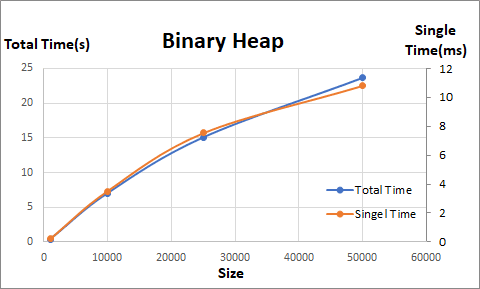
\includegraphics[width=0.5\textwidth]{1.png}
    }
    \subfloat[Fibonacci]
    {
        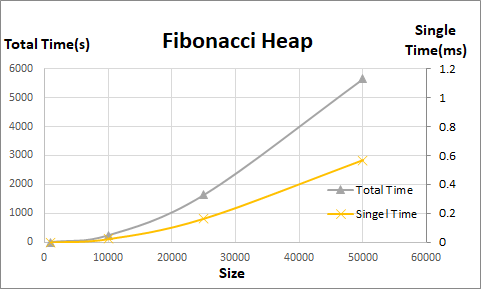
\includegraphics[width=0.5\textwidth]{2.png}
    }\\
    \subfloat[Binomial]
    {
        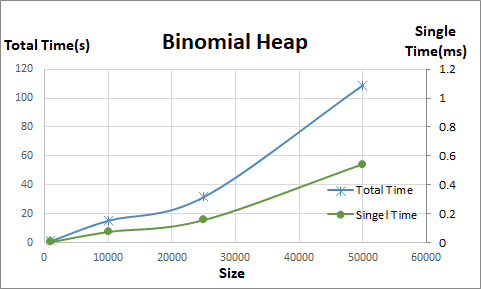
\includegraphics[width=0.5\textwidth]{3.png}
    }
    \subfloat[Leftist]
    {
        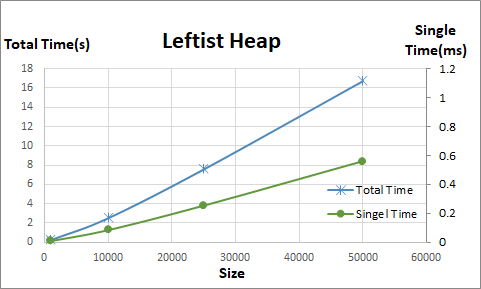
\includegraphics[width=0.5\textwidth]{ww.png}
    }
    \caption{Diagram for the Running Time Versus Input Sizes}
\end{figure}
Obviously, with input size increasing, the time increases too. And among our four heap optimization, leftist heap is the best in this test.   
\subsection{Test the USA Road Networks}
This test data is given on the \href{http://www.dis.uniroma1.it/challenge9/download.shtml}{website}. 

It's worth noting that the time shown below in a unit of milliseconds and the test environment is MacbookPro 14 m1 pro. 
\begin{figure}[H]
    \centering
    \subfloat[USA(23,947,347 nodes and 58,333,344 arcs)]
    {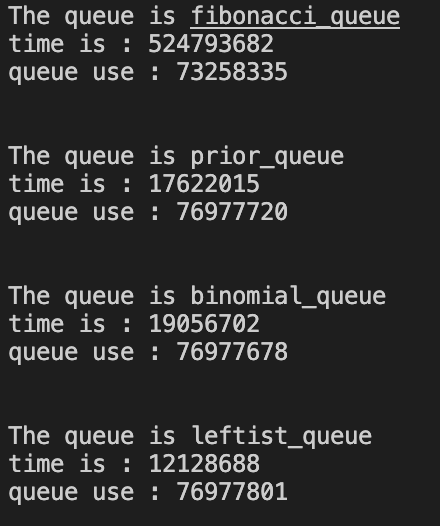
\includegraphics[width=0.4\textwidth]{00.png}}
    \subfloat[COL(435,666 nodes and 1,057,066 arcs)]
    {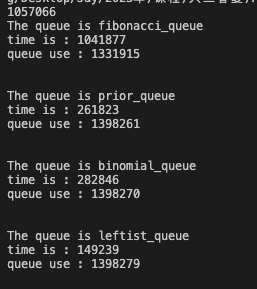
\includegraphics[width=0.4\textwidth]{col.png}}
    % \caption{}
\end{figure}
\begin{figure}[H]
    \centering
    \subfloat[FLA(1,070,376 nodes and 2,712,798 arcs)]
    {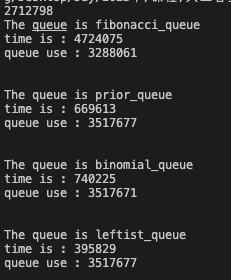
\includegraphics[width=0.4\textwidth]{fla.png}}
    \subfloat[E(3,598,623 nodes and 3,598,623 arcs)]
    {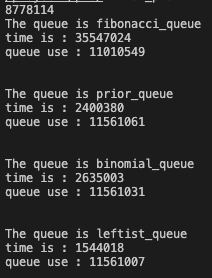
\includegraphics[width=0.4\textwidth]{e.png}}
\end{figure}
\begin{figure}[H]
    \centering
    \subfloat[CAL(1,890,815 nodes and 1,890,815 arcs)]
    {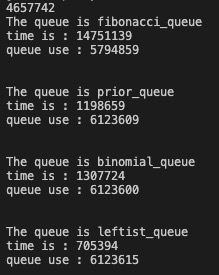
\includegraphics[width=0.4\textwidth]{cal.png}}
    \subfloat[LKS(2,758,119 nodes and 6,885,658 arcs)]
    {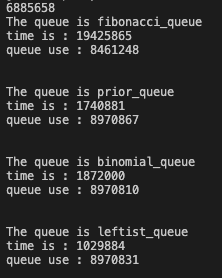
\includegraphics[width=0.4\textwidth]{lks.png}}
\end{figure}
\begin{figure}[H]
    \centering
    \subfloat[NE(1,524,453 nodes and 1,524,453 arcs)]
    {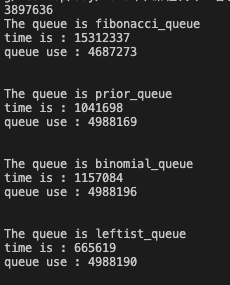
\includegraphics[width=0.4\textwidth]{ne.png}}
    \subfloat[NW(1,524,453 nodes and 1,524,453 arcs)]
    {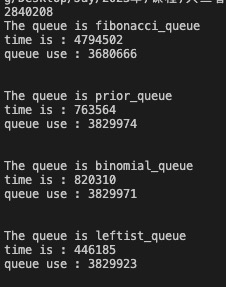
\includegraphics[width=0.4\textwidth]{nw.jpg}}
\end{figure}
\begin{figure}[H]
    \centering
    \subfloat[W(6,262,104 nodes and 6,262,104 arcs)]
    {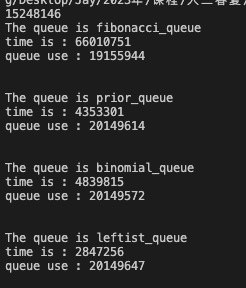
\includegraphics[width=0.4\textwidth]{w.jpg}}
    \subfloat[CTR(14,081,816 nodes and 14,081,816 arcs)]
    {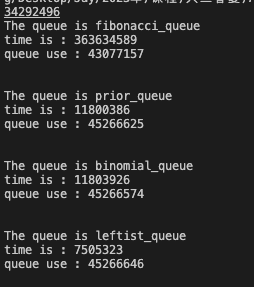
\includegraphics[width=0.4\textwidth]{ctr.png}}
    \caption{Test Provided Data Sets}
\end{figure}
And we plot all situations into one diagram. (Note that since the time of Fibonacci is far greater than the other three heaps, we use a different axis for Fibonacci heap.)
\begin{figure}[H]
    \centering
    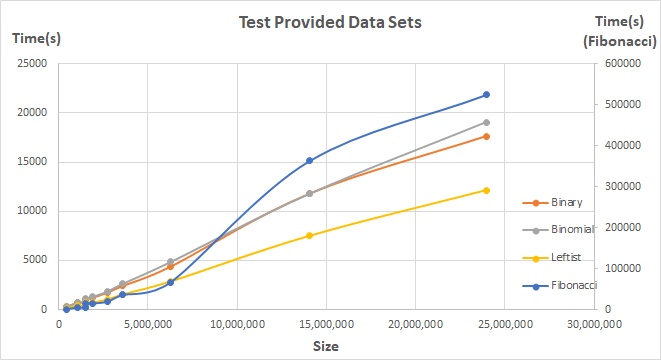
\includegraphics[width=0.75\textwidth]{ok.png}
    \caption{Test Provided Data Sets}
\end{figure}
From the diagram, we can draw similar conclusion as 3.1, which is that the leftist heap has the best performance while Fibonacci heap is worse than other heaps.
\section{Analysis and Comments}

\subsection{Time Complexity}
\begin{itemize}
    \item \textbf{For Dijkstra's algorithm with a binary heap, a binomial heap or a leftist heap}

    Time complexity of ${O((E + V) \log V)}$, where $E$ is the number of edges and $V$ is the number of vertices in the graph.
    
    In this case, the algorithm maintains a heap of vertices by their distance from the source vertex.  The insertion of a new vertex requires ${O(\log V)}$ time complexity in the worst case, while the decrease key operation and the extraction of the minimum vertex require ${O(\log V)}$ time complexity each.  Since these operations are performed a maximum of $E + V$ times, the total time complexity is ${O((E + V) \log V)}$.
    \item \textbf{For Dijkstra's algorithm with a Fibonacci heap}

    Time complexity of ${O(E + V \log V)}$, where $E$ is the number of edges and $V$ is the number of vertices in the graph. 

    To take advantage of the decrease key operation in Dijkstra's algorithm, you need to maintain a reference to each vertex in the heap. The decrease key operation in Fibonacci heap has an amortized time complexity of ${O(1)}$, which means that it is a constant-time operation on average.

    In this case, the algorithm maintains a Fibonacci heap of vertices by their distance from the source vertex. The insertion of a new vertex and the decrease key operation both have an amortized time complexity of ${O(1)}$, while the extraction of the minimum vertex has an amortized time complexity of ${O(\log V)}$. Since these operations are performed a maximum of $E + V$ times, the total time complexity is ${O(E + V \log V)}$. In detail, building the heap is $O(V)$, extracting minimum vertex is $O(V\log V)$, updating the distances is $O(E)$, so the result is ${O(E + V \log V)}$.

    Besides, although STL
    \item \textbf{Summary}
    
    As we can see, in theory, Fibonacci heap has a better time complexity than binary heap for some operations, including decrease key and merge, especially for sparse graphs with many unreachable vertices.   
    
    However, in practice, Fibonacci heap may not always be the best choice for Dijkstra's algorithm due to its higher constant factor and more complex implementation compared to binary heap, which can explain why in our test the performance of Fibonacci heap is much worse than the binary heap. 
    
    The choice between Fibonacci heap and binary heap should depend on the specific characteristics of the graph and the performance requirements of the application.
\end{itemize}
\subsection{Space Complexity}
In Dijkstra with heap optimization, space complexity is $O(V + E)$, where $E$ is the number of edges and $V$ is the number of vertices in the graph.   

In this case, the algorithm maintains a heap of vertices by their distance from the source vertex. The heap requires space proportional to the number of vertices, which is $O(V)$. Additionally, the algorithm maintains an adjacency list to store the edges and their weights. The space required for the adjacency list or matrix is $O(E)$. Besides, for Fibonacci heap, we need an additional array to record the position stored in the  heap of each node, so that we can call \verb|DecreaseKey| without searching for the position, which also cost $O(V)$. Therefore, the total space complexity is $O(V + E)$. 

\section{Author list}
The code and report are finished by all of us.


JieFeng Hu finish the code.\\
Jiajun Qin finish the report.\\
Wenjie Huang finish the PPT of the presentation.

\section*{Declaration}
We hereby declare that all the work done in this project titled "Shortest Path Algorithm with Heaps" is of our independent effort as a group.

\section{Signatures}

We hereby declare that all the work done in this project titled ”Shortest Path Algorithm with Heaps” is of our independent effort as a group.


\vskip 1.5in
\newpage

%%%% References 
%%% bibliographystyle: is the referece style, such as plain, abbrv et al. 
%%% bibliography: the file.bib;
\bibliographystyle{abbrv}
%\bibliographystyle{plain}
\bibliography{ads}


\appendix 
\section{Source Code (if required)}
% \begin{lstlisting}[basicstyle = \small\JB]
%     #include <iostream>
%     #include<fstream>
%     #include<vector>
%     #include<queue>
%     #include<time.h>
%     #include<random>
%     using namespace std;
%     long queue_use;
%     long time_second;
%     const int INF = 0x3f3f3f3f;
%     // 2^30
%     const long CAPITAL = 1073741824;
    
%     // 点的定义,尽可能简洁,name 是 node 的位置
%     // dis是距离源点的距离
%     struct node{
%         int name;
%         int dis;
%         node(int n=-1,int d=INF){name=n;dis=d;}
%         // 需要重载比较符号
%         // 本来是最大堆,这样就是最小堆了
%         bool operator <( const node &r )const{
%             return  dis < r.dis ;
%         }
%         bool operator ==( const node &r )const{
%             return dis == r.dis;
%         }
%         bool operator !=( const node &r )const{
%             return dis != r.dis;
%         }
%     };
    
%     // 点的定义,尽可能简洁,name是node的位置
%     // dis是距离源点的距离
%     // pri是专门改过大小的,把最大堆变成最小堆
%     struct node_pri{
%         int name;
%         int dis;
%         node_pri(int n=-1,int d=INF){name=n;dis=d;}
%         // 需要重载比较符号
%         // 本来是最大堆,这样就是最小堆了
%         bool operator <( const node_pri &r )const{
%             return  dis > r.dis ;
%         }
%         bool operator ==( const node_pri &r )const{
%             return dis == r.dis;
%         }
%         bool operator !=( const node_pri &r )const{
%             return dis != r.dis;
%         }
%     };
    
%     // 边的定义,尽可能简洁,仅有目的地和距离
%     struct edge{
%         int mute;
%         int distance;
%         edge(int e,int d){mute=e;distance=d;}
%     };
    
%     /****************************************************斐波那契堆部分*****************************************************/
%     struct FibNode{
%             // 内容是key,格式为node
%             node key;
%             // 左右兄的双向链表指针
%             FibNode* rbro;
%             FibNode* lbro;
%             // 父子的指针
%             FibNode* father;
%             FibNode* child;
%             // 节点的度
%             int degree;
%             // 是否失去过子
%             bool mark;
%             void Init();
%     };
    
%     // 对点进行初始化
%     void FibNode::Init(){
%         // 左右兄都指向自己
%         rbro = lbro = this;
%         // 父子都为空
%         father = child = NULL;
%         // 节点的度为0
%         degree = 0;
%         // makr 也为0
%         mark = false;
%     }
    
%     class FibHeap{
%         public:
%             FibHeap(){min=NULL;number=0;}
%             FibNode* push(node a);
%             node pop();
%             bool empty();
%             void decrease( FibNode* x, int k );
%         private:
%             // 指向最小的节点
%             FibNode* min;
%             // 树内的所有的点的个数
%             int number;
%             void cut( FibNode* x, FibNode* y );
%             void cascading_cut( FibNode* y );
%             void consolidate();
%     };
    
%     FibNode* cat_pointer( FibNode* a, FibNode* b){
%         // 如果其中一个是空的
%         // 直接返回
%         if( a == NULL ) return b;
%         if( b == NULL ) return a;
%         // 定义一个暂时的指针
%         FibNode* temp;
%         // 将两个双向链表连接起来
%         temp = a->rbro;
%         a->rbro = b->rbro;
%         b->rbro->lbro = a;
%         b->rbro = temp;
%         temp->lbro = b;
%         return a;
%     }
    
%     // 插入操作
%     FibNode* FibHeap::push( node a ){
%         // 新请求一个空间来存放
%         FibNode* x = (FibNode*)malloc(sizeof(FibNode));
%         // 初始化并赋值
%         x->Init();
%         x->key = a;
%         // 讲x插入到森林中
%         // 如果为空就直接插进去
%         if( min == NULL )   min = x;
%         // 否则就插入到链表中
%         else{
%             // 插入到root的双向链表中
%             cat_pointer( min , x );
%             // 更新min
%             if( x->key < min->key ) min = x;
%         }
%         // 更新number
%         number ++;
%         // 返回指针方便查找
%         return x;
%     }
    
%     // 把点从双向链表中脱除
%     void delete_pointer( FibNode* a ){
%         // 左右子链互连
%         a->lbro->rbro = a->rbro;
%         a->rbro->lbro = a->lbro;
%         // 左右兄连自己
%         a->rbro = a->lbro = a;
%         a->father = NULL;
%     }
    
%     // 将一个点链接到另一个的子链表中
%     void heap_link( FibNode* child, FibNode* father ){
%         // child 脱离原来的链表
%         delete_pointer( child );
%         // 把child纳入farther的子链表
%         father->child = cat_pointer( father->child, child );
%         // 更新child的father和father的degree
%         father->degree ++;
%         child->father = father;
%         return;
%     }
    
%     // 调整堆的性质
%     void FibHeap::consolidate(){
%         // 如果min是null则不用调整
%         if( min == NULL )   return ;
%         // 创建新的堆来缓冲
%         FibNode* A[number];
%         // 清理内存
%         for( int i=0; i<number; i++ )   A[i] = NULL;
%         // 建立暂时的指针
%         FibNode* now_pointer = min;
%         // 遍历所有的root双向链表
%         do{
%             // 建立临时变量
%             FibNode* x = now_pointer;
%             int degree = x->degree;
%             // 开始找A中合适的区域
%             while( A[degree] != NULL ){
%                 // 建立临时变了
%                 FibNode* y = A[degree];
%                 // 判断谁的值更小做父
%                 if( y->key < x->key ){
%                     // 交换
%                     FibNode* temp = x;
%                     x = y;
%                     y = temp;
%                 }
%                 // 链接两个
%                 heap_link( y, x );
%                 // 原来的清理一下
%                 A[degree] = NULL;
%                 // 更新degree   
%                 degree++;
%             }
%             // 找到了放入
%             A[degree] = x;
%         }while( now_pointer != min );
%         // 抹去原来的森林
%         min = NULL;
%         // 重新调整森林
%         for( int i=0; i<number; i++ ){
%             if( A[i] != NULL ){
%                 // 如果min还没有的话,就作为min
%                 if( min == NULL )   min = A[i];
%                 // 否则就加入min的双向链表
%                 else{
%                     cat_pointer( min, A[i] );
%                     // 更新min
%                     if( A[i]->key < min->key )  min = A[i];
%                 }
%             }
%         }
%         return;
%     }
    
%     // 弹出最小的点
%     node FibHeap::pop(){
%         // 先把min分离出来
%         FibNode* z = min;
%         // 如果堆不为空
%         if( z != NULL ){
%             // 把z的子都转移到root上
%             while( z->degree != 0 ){
%                 // 标记要分离的子
%                 FibNode* child = z->child;
%                 // 子的指针指向null或右兄
%                 if( z->degree == 1 )    z->child = NULL;
%                 else    z->child = z->child->rbro;
%                 // 子脱离
%                 delete_pointer( child );
%                 // z的degree更新
%                 z->degree --;
%                 // 将子链接到主链上
%                 cat_pointer( min, child );
%             }
%             // 先判断min
%             if( z->rbro == z )  min=NULL;
%             else    min = z->rbro;
%             // 把z移除
%             delete_pointer( z );
%             // 调整
%             consolidate();
%             // 更新number
%             number --;
%         }
%         return z->key;
%     }
    
%     // 辅助函数,把x提取到最上面,调整最小堆性质
%     void FibHeap::cut( FibNode* x, FibNode* y ){
%         // 判断一下y的子节点是只有一个x还是还有其他的
%         if( y->degree == 1 )    y->child = NULL;
%         else    y->child = x->rbro;
%         // 更新y的degree
%         y->degree --;
%         // 把x从y中提取出来
%         delete_pointer( x );
%         // 把x加入到主链表中
%         cat_pointer( min , x );
%         x->mark = false;
%     }
    
%     // 辅助函数,调整最小堆性质
%     void FibHeap::cascading_cut( FibNode* y ){
%         // 建立临时变量
%         FibNode* z = y->father;
%         // 如果y不在主链表里
%         if( z != NULL ){
%             // 如果y的mark是否
%             if( y->mark == false )  y->mark = true;// 调整过来
%             else{
%                 // 递归做cut
%                 cut( y , z );
%                 cascading_cut( z ); 
%             }
%         }
%     }
    
%     // 减少指定指针的值
%     void FibHeap::decrease( FibNode* x, int k ){
%         // 只能减少
%         if( k > x->key.dis )    return;
%         // 更新
%         x->key.dis = k;
%         // 建立临时变量
%         FibNode* y = x->father;
%         // 如果x不是顶层,且x比y的值更小
%         if( y!= NULL && x->key < y->key ){
%             // cut和cascading-cut两个操作
%             cut( x, y );
%             cascading_cut( y );
%         }
%         // 如果x的值比min小,就代替min
%         if( x->key < min->key ) min = x;
%     }
    
%     bool FibHeap::empty(){
%         return number==0;
%     }
%     /****************************************************斐波那契堆部分结束***************************************************/
    
%     /******************************************************二项堆部分*******************************************************/
%     // binary heap的点
%     struct binonode{
%         // 节点的key为node_pri,因为堆是最大堆
%         node key;
%         // 父节点,左右子节点
%         binonode* nsibil;
%         binonode* lchild;
%     };
    
%     // binary heap
%     class binoheap{
%         public:
%             binoheap(){number=0;for(int i=0;i<30;i++)   forest[i]=NULL;}
%             node pop();
%             bool empty();
%             void push( node in );
%             void combineForest( binoheap H2 );
%             binonode* combineTree( binonode* T1, binonode* T2 );
%         private:
%             // 堆的个数
%             int number;
%             // 森林的数组
%             binonode* forest[30];
%     };
    
%     // 合并两个树
%     binonode* binoheap::combineTree( binonode* T1, binonode* T2 ){
%         // key小的做父
%         if( T2->key < T1->key ) return combineTree( T2, T1 );
%         // 把T2作为T1的子
%         // T2变成T1的最左边的儿子
%         T2->nsibil = T1->lchild;
%         T1->lchild = T2;
%         // 返回父
%         return T1;
%     }
    
%     // 合并两个森林,其中一个是这个类森林
%     void binoheap::combineForest( binoheap H2 ){
%         // 定义临时变量
%         binonode* T1;
%         binonode* T2;
%         binonode* Carry=NULL;
%         // 如果超出范围就要报错
%         if( number + H2.number > CAPITAL )   exit(1);
%         // 准备把所有都转移到T1上
%         number += H2.number;
%         // 最大的上限是lognumber
%         int i,j;
%         for( i=0,j=1; j<=number; i++,j*=2 ){
%             // 截取T1和T2当前的tree
%             T1 = forest[i];T2 = H2.forest[i];
%             // 人造三位二进制判定是否为0
%             switch ( 4*(!!Carry) + 2*(!!T2) + (!!T1) )
%             {
%             // 全0就不用任何操作,因为三个都没有任何东西
%             case 0:break;
%             // 001 只有T1不为NULL,直接跳过就行
%             case 1:break;
%             // 010 只有T2有,要转到T1去
%             case 2:forest[i]=T2;H2.forest[i]=NULL;break;
%             // 011 T1T2都有,需要融合,要到下一层
%             case 3:Carry=combineTree( T1, T2 );forest[i]=H2.forest[i]=NULL;break;
%             // 100 只有carry有,驾到这里
%             case 4:forest[i]=Carry;Carry=NULL;break;
%             // 101,只有Carry和T1有,融合到下一层
%             case 5:Carry=combineTree(Carry,T1);forest[i]=NULL;break;
%             // 110,只有Carry和T2有,融合到下一层
%             case 6:Carry=combineTree(Carry,T2);H2.forest[i]=NULL;break;
%             // 111 三个都有Carry给森林,T1T2融合下一层
%             case 7:forest[i]=Carry;Carry=combineTree(T1,T2);H2.forest[i]=NULL;break;
%             }
%         }
%         return;
%     }
    
%     // 插入一个节点
%     void binoheap::push( node in ){
%         // 如果binoheap是空的,直接加到1的地方就行
%         // 创建新的点
%         binonode* newNode = (binonode*)malloc(sizeof(binonode));
%         // 初始化
%         newNode->lchild = NULL;newNode->nsibil = NULL;
%         // 赋值
%         newNode->key = in;
%         // 如果森林是空的,可以直接加到0里去
%         if( number == 0 ){
%             forest[0] = newNode;
%             number ++;
%             return;
%         }
%         else{
%             // 建立一个只有这个点的森林融合
%             binoheap temp;
%             temp.number=1;
%             temp.forest[0] = newNode;
%             combineForest( temp );
%         }
%         // 结束
%         return;
%     }
    
%     // 推出最小点
%     node binoheap::pop(){
%         // 新建一个承载子节点的堆
%         binoheap Delete;
%         // 建立临时变量
%         binonode* DeleteTree;
%         binonode* OldRoot;
%         // 即将推出去的最小的值
%         node MinItem;
%         // 如果是空的直接报错
%         if( number == 0 )   exit(1);
%         // 定义临时变量
%         int i,j,MinTree;
%         // 遍历所有根找最小的值所在的树的根点
%         for( int i=0; i<30; i++ ){
%             // 这个点即不为NULL,又比MinItrm小
%             if( forest[i] != NULL && forest[i]->key < MinItem ){
%                 // MinItem就是这个,更新
%                 MinItem = forest[i]->key;
%                 MinTree = i;
%             }
%         }
%         // 确定删除的点
%         DeleteTree = forest[MinTree];
%         // 在森林中删除
%         forest[MinTree] = NULL;
%         // 准备转移
%         OldRoot = DeleteTree;
%         DeleteTree = DeleteTree->lchild;
%         // 解放原来的节点
%         free(OldRoot);
%         // 点的数量就是2的幂次方减去删去的
%         Delete.number =(1 << MinTree)-1;
%         // 开始加值
%         for( j=MinTree-1; j>=0; j-- ){
%             Delete.forest[j] = DeleteTree;
%             DeleteTree = DeleteTree->nsibil;
%             Delete.forest[j]->nsibil = NULL;
%         }
%         // 融合
%         // 先更新原来的值
%         number -= ( Delete.number + 1 );
%         // 再融合
%         combineForest( Delete );
%         // 返回最小值
%         return MinItem;
%     }
    
%     // 测试是否还有内容
%     bool binoheap::empty(){
%         return number==0;
%     }
    
%     /******************************************************二项堆部分结束****************************************************/
    
%     /******************************************************左倾斜堆部分******************************************************/
%     // Lefist heap node 的点结构
%     struct LefistNode{
%         node key;
%         // Npl属性,用来调整堆的性质
%         int Npl;
%         // 左右的孩子
%         LefistNode* lchild;
%         LefistNode* rchild;
%     };
    
%     // Leftist heap 
%     class LefistTree{
%         public:
%             LefistTree(){tree=NULL;number=0;}
%             node pop();
%             void push( node in );
%             bool empty();
%             LefistNode* Merge( LefistNode* H1, LefistNode* H2 );
%         private:
%             LefistNode* Merge_( LefistNode* H1, LefistNode* H2 );
%             int number;
%             LefistNode* tree;
%     };
    
%     // 辅助函数,融合两个树的实际操作
%     LefistNode* LefistTree::Merge_( LefistNode* H1, LefistNode* H2 ){
%         // single Node,直接融合
%         if( H1->lchild == NULL )    H1->lchild = H2;
%         // 否则就要转化一下
%         else{
%             // 融合
%             H1->rchild = Merge( H1->rchild, H2 );
%             // 转化孩子
%             if( H1->lchild->Npl < H1->rchild->Npl ){
%                 LefistNode* temp = H1->lchild;
%                 H1->lchild = H1->rchild;
%                 H1->rchild = temp;
%             }
%             // 更新Npl
%             H1->Npl = H1->rchild->Npl + 1;
%         }
%         // 返回
%         return H1;
%     }
    
%     // 融合两个树
%     LefistNode* LefistTree::Merge( LefistNode* H1, LefistNode* H2 ){
%         // 判断一下需不需要融合,如果一方为null直接返回就OK
%         if( H1 == NULL )    return H2;
%         if( H2 == NULL )    return H1;
%         // 判断怎么链接
%         if( H1->key < H2->key ) return Merge_( H1, H2 );
%         else    return Merge_( H2, H1 );
%     }
    
%     node LefistTree::pop(){
%         // 找到最小的点
%         LefistNode* Min = tree;
%         // 建立临时变量
%         LefistNode* Ltree = tree->lchild;
%         LefistNode* Rtree = tree->rchild;
%         // 删除tree建立新的tree
%         tree = Merge( Ltree, Rtree );
%         // 返回最小的
%         return Min->key;
%     }
    
%     // 压入元素到堆里
%     void LefistTree::push( node in ){
%         // 就是把新的作为新树压进去
%         // 建立新的点
%         LefistNode* newNode = (LefistNode*)malloc(sizeof(LefistNode));
%         newNode->key = in;
%         newNode->lchild = newNode->rchild = NULL;
%         newNode->Npl = 1;
%         // 把新的点压进去
%         tree = Merge( tree, newNode );
%         return;
%     }
    
%     // 判断是否为空
%     bool LefistTree::empty(){
%         return tree==NULL;
%     }
    
%     /******************************************************左倾斜堆部分结束***************************************************/
    
    
%     // vis dis和 pre即是否被检测过,前一个点用全局来表示,否则用queue无法读取
%     int* vis;
%     int* pre;
%     int* dis;
%     // nodeLib 是用来存储不同点的指针的,便于在O(1)内找到
%     FibNode** nodeLib;
    
%     // 地图用vector来存储
%     vector<edge>* map;
    
%     // 初始化
%     void Init(int NodeNum){
%         // 初始化vis和pre
%         if( vis )   free(vis);
%         if( pre )   free(pre);
%         if( dis )   free(dis);
%         // vis的初始化都是没vis过
%         vis = (int*)malloc(sizeof(int)*NodeNum);
%         // pre的初始化是-1.即没有
%         pre = (int*)malloc(sizeof(int)*NodeNum);
%         // dis的初始化是无穷大
%         dis = (int*)malloc(sizeof(int)*NodeNum);
%         for( int i=0; i<NodeNum; i++){
%             vis[i]=0;
%             pre[i]=-1;
%             dis[i]=INF;
%         } 
%         return;
%     }
    
%     // Dijkstra算法实现,返回double形式的运行时间
%     double Dijkstra_fib(int source, FibHeap q ) {
%         // 计时,计次数
%         clock_t start, end;
%         start = clock();
    
%         // 函数实现部分
%     /*----------------------------------------------------------------------------------------*/
%         // 起点为0
%         // 压入第一个点
%         q.push(node(source,0));
%         queue_use++;
%         // 第一个点的map定为0
%         dis[source] = 0;
%         node Temp;
%         // 只要还没遍历完
%         while(!q.empty()){
%             // 压出距离最近的一个
%             Temp = q.pop();
%             queue_use += 2;
%             // 查看是否遍历过  
%             if( vis[Temp.name] ) continue;
%             else    vis[Temp.name] = 1;
%             // 开始逐个找该点的边
%             int num = map[Temp.name].size();
%             // 逐个找边
%             for(int i=0; i<num; i++ ){
%                 // 这个边是当前操作的边
%                 edge tmp = map[Temp.name][i];
%                 // 边的连接的点
%                 int mute = tmp.mute;
%                 // 如果边也被遍历过,说明肯定无法再有优化,直接跳过
%                 if( vis[mute] ) continue;
%                 // 边的distance
%                 int distance = tmp.distance;
%                 // 如果从这个点走可以有优化
%                 if( dis[mute] > dis[Temp.name] + distance ){
%                     // 如果是不在堆里,即还是INF的
%                     if( dis[mute] == INF ){
%                         // 更新距离
%                         dis[mute] = dis[Temp.name] + distance;
%                         // 加入堆
%                         // 加入地图
%                         nodeLib[mute] = q.push(node(mute,dis[mute]));
%                     }
%                     // 如果在堆里,就直接更新堆
%                     else{
%                         // 更新距离
%                         dis[mute] = dis[Temp.name] + distance;
%                         // 在地图中找到指针,并更新
%                         q.decrease( nodeLib[mute], dis[mute] );
%                     }
                    
%                     queue_use++;
%                 }
%             }
%         }
    
%     /*----------------------------------------------------------------------------------------*/
%         end = clock();
%         // cout << "begin " << start << " end " << end << endl;
%         return (double) (end - start);
%     }
    
%     // Dijkstra算法实现,返回double形式的运行时间
%     // T作为一个heap。有几个基础的功能
%     double Dijkstra(int source, priority_queue<node_pri> q ) {
%         // 计时,计次数
%         clock_t start, end;
%         start = clock();
    
%         // 函数实现部分
%     /*----------------------------------------------------------------------------------------*/
%         // 起点为0
%         // 压入第一个点
%         q.push(node_pri(source,0));
%         queue_use++;
%         // 第一个点的map定为0
%         dis[source] = 0;
%         node_pri Temp;
%         // 只要还没遍历完
%         while(!q.empty()){
%             // 压出距离最近的一个
%             Temp = q.top();
%             q.pop();
%             queue_use += 2;
%             // 查看是否遍历过  
%             if( vis[Temp.name] ) continue;
%             else    vis[Temp.name] = 1;
%             // 开始逐个找该点的边
%             int num = map[Temp.name].size();
%             // 逐个找边
%             for(int i=0; i<num; i++ ){
%                 // 这个边是当前操作的边
%                 edge tmp = map[Temp.name][i];
%                 // 边的连接的点
%                 int mute = tmp.mute;
%                 // 如果边也被遍历过,说明肯定无法再有优化,直接跳过
%                 if( vis[mute] ) continue;
%                 // 边的distance
%                 int distance = tmp.distance;
%                 // 如果从这个点走可以有优化
%                 if( dis[mute] > dis[Temp.name] + distance ){
%                     dis[mute] = dis[Temp.name] + distance;
%                     q.push(node_pri(mute,dis[mute]));
%                     queue_use++;
%                 }
%             }
%         }
    
%     /*----------------------------------------------------------------------------------------*/
%         end = clock();
%         // cout << "begin " << start << " end " << end << endl;
%         return (double) (end - start);
%     }
    
%     // Dijkstra算法实现,返回double形式的运行时间
%     // T作为一个heap。有几个基础的功能
%     template<class T>
%     double Dijkstra_bino(int source, T q ) {
%         // 计时,计次数
%         clock_t start, end;
%         start = clock();
    
%         // 函数实现部分
%     /*----------------------------------------------------------------------------------------*/
%         // 起点为0
%         // 压入第一个点
%         q.push(node(source,0));
%         queue_use++;
%         // 第一个点的map定为0
%         dis[source] = 0;
%         node Temp;
%         // 只要还没遍历完
%         while(!q.empty()){
%             // 压出距离最近的一个
%             Temp = q.pop();
%             queue_use += 2;
%             // 查看是否遍历过  
%             if( vis[Temp.name] ) continue;
%             else    vis[Temp.name] = 1;
%             // 开始逐个找该点的边
%             int num = map[Temp.name].size();
%             // 逐个找边
%             for(int i=0; i<num; i++ ){
%                 // 这个边是当前操作的边
%                 edge tmp = map[Temp.name][i];
%                 // 边的连接的点
%                 int mute = tmp.mute;
%                 // 如果边也被遍历过,说明肯定无法再有优化,直接跳过
%                 if( vis[mute] ) continue;
%                 // 边的distance
%                 int distance = tmp.distance;
%                 // 如果从这个点走可以有优化
%                 if( dis[mute] > dis[Temp.name] + distance ){
%                     dis[mute] = dis[Temp.name] + distance;
%                     q.push(node(mute,dis[mute]));
%                     queue_use++;
%                 }
%             }
%         }
    
%     /*----------------------------------------------------------------------------------------*/
%         end = clock();
%         // cout << "begin " << start << " end " << end << endl;
%         return (double) (end - start);
%     }
    
    
%     // 读取地图文件
%     int readFile( string filePath ){
%         // 读取数据阶段
%         ifstream mapFile;
%         // cout << "begin" << endl;
%         // if(argv[1][0] == 'a' )  mapFile.open("./USA-road-d.E.gr",ios::in);
%         // else    mapFile.open("./USA-road-d.NY.gr",ios::in);
%         mapFile.open(filePath,ios::in);
%         // 把前面几行注释读取掉
%         char l[100];
%         for( int i=0; i<4; i++ ){
%             mapFile.getline(l,100);
%         }
%         // 读取关键信息 
%         char type;char sign[3];int num_1,num_2;
%         // 读取文件最开始
%         mapFile >> type >> sign >>num_1 >> num_2;
%         // 再读无用的注视
%         mapFile.getline(l,100);
%         mapFile.getline(l,100);
%         mapFile.getline(l,100);
%         // 构建数据结构
%         // 构建地图
%         // cout << sizeof(vector<edge>)*num_1 << endl;
%         map = (vector<edge>*)std::malloc(sizeof(vector<edge>)*num_1);
    
%         // 一共有num_2个线
%         char type_2;
%         int node_1,node_2,length;
%         for( int i=0; i<num_2; i++ ){
%             mapFile >> type_2 >> node_1 >> node_2 >> length;
%             if( type_2 != 'a') return 1;
%             map[node_1].push_back(edge(node_2,length));
%         }
%         cout << num_2 << endl;
%         // cout << "end" << endl;
%         mapFile.close();
%         // 读取数据结束
%         // 数据以edge的形式存储在map里
%         return num_1;
%     }
    
%     int main(){
    
%         // 读取文件内的路
%         int node_number;
%         // 读取路径的相对路径
%         string filePath = "./USA-road-d.USA.gr";
%         node_number = readFile(filePath);
        
%         // 跑几个随机点
%         int test_number = 1;
    
%     // 测试斐波那契堆
%     // 测试数据 USA地图,随机找1000个点,并找出其所有的通路及最短路径
%     // 测试输出 queue的用的次数,还有时间
%     /*----------------------------------------------------------------------------------------*/
    
%         time_second = 0;
%         queue_use = 0;
%         for( int i=0; i<test_number; i++ ){
%             // 开始测试
%             Init(node_number);
%             nodeLib = (FibNode**)malloc(sizeof(FibNode*)*node_number);
%             // 先用prior_queue试一试
%             FibHeap Fib;
%             time_second += Dijkstra_fib(i*100+2301,Fib);
%         }
%         cout << "The queue is fibonacci_queue" << endl;
%         cout << "time is : " << time_second << endl;
%         cout << "queue use : " << queue_use << endl;
%         cout << "\n" << endl;
    
%     /*----------------------------------------------------------------------------------------*/
    
%     // 测试std::prior_queue
%     // 测试数据 USA地图,随机找1000个点,并找出其所有的通路及最短路径
%     // 测试输出 queue的用的次数,还有时间
%     /*----------------------------------------------------------------------------------------*/
    
%         time_second = 0;
%         queue_use = 0;
%         for( int i=0; i<test_number; i++ ){
%             // 开始测试
%             Init(node_number);
%             // 先用prior_queue试一试
%             priority_queue<node_pri> prior;
%             time_second += Dijkstra(i*100+2301,prior);
%         }
%         cout << "The queue is prior_queue" << endl;
%         cout << "time is : " << time_second << endl;
%         cout << "queue use : " << queue_use << endl;
%         cout << "\n" << endl;
    
%     /*----------------------------------------------------------------------------------------*/
    
    
%     // 测试binomal heap
%     // 测试数据 USA地图,随机找1000个点,并找出其所有的通路及最短路径
%     // 测试输出 queue的用的次数,还有时间
%     /*----------------------------------------------------------------------------------------*/
    
%         time_second = 0;
%         queue_use = 0;
%         for( int i=0; i<test_number; i++ ){
%             // 开始测试
%             Init(node_number);
%             // 先用prior_queue试一试
%             binoheap bino;
%             time_second += Dijkstra_bino(i*100+2301,bino);
%         }
%         cout << "The queue is binomial_queue" << endl;
%         cout << "time is : " << time_second << endl;
%         cout << "queue use : " << queue_use << endl;
%         cout << "\n" << endl;
    
%     /*----------------------------------------------------------------------------------------*/
    
%     // 测试leftist heap
%     // 测试数据 USA地图,随机找1000个点,并找出其所有的通路及最短路径
%     // 测试输出 queue的用的次数,还有时间
%     /*----------------------------------------------------------------------------------------*/
    
%         time_second = 0;
%         queue_use = 0;
%         for( int i=0; i<test_number; i++ ){
%             // 开始测试
%             Init(node_number);
%             // 先用prior_queue试一试
%             LefistTree leftist;
%             time_second += Dijkstra_bino(i*100+2301,leftist);
%         }
%         cout << "The queue is leftist_queue" << endl;
%         cout << "time is : " << time_second << endl;
%         cout << "queue use : " << queue_use << endl;
%         cout << "\n" << endl;
    
%     /*----------------------------------------------------------------------------------------*/
%         return 0;
%     }
% \end{lstlisting}
\lstinputlisting[basicstyle = \small\JB, language=C++]{Final_pro2.cpp} 

\end{CJK*} 
\end{document}
\newpage



